\section{Social Security in Rich OECD Countries}\label{sec:oecd}\label{sec:quant:OECD}
In order to study the determinants of pensions, we now calibrate the model to three rich OECD economies that differ markedly in pension spending, demography, income inequality, voting patterns and pension design: the U.S., France and the UK. In these economies nearly every worker qualifies for a contributory pension, so we set informality aside and the design reduces to one dimension, the extent to which benefits are earnings-related.\footnote{\textcite{WhitmanRa1} estimate that about 4\% of individuals aged 62--84 in the U.S.\ in 2010 would never collect Social Security, most of them for lack of the 40 quarters of covered earnings needed to qualify.} To explore what characteristics shape pensions, savings rates, and labor supply, we simulate counterfactual economies that are calibrated to the U.S. with one characteristic changed at a time. 

\smalltitle{Calibration.}
We calibrate the model without informal households on men aged 25 to 60, with three income groups per country and 2020 as the calibration year; appendix \ref{app:US} documents the household surveys, the parameters of each income group and the sources. The design $\theta$ is identified from the OECD's replacement rates at mean and half-mean income, so the first two groups are cut to have mean incomes of half the mean and the mean, and the rest of the population forms the high income group. France's system is fully Bismarckian, $\theta = 1$ at any cuts, so we group French households at the U.S.\ income percentiles instead, which puts the two countries' household types in one-to-one correspondence for the counterfactuals below. As for Argentina (appendix \ref{app:EPH}), relative income pins down each group's combination of productivity and taste for leisure, $\eta_i^{1+\xi}/X_i^{\xi}$, and nothing more, so we take $X_i = X$ common across groups and let each country's observed average workweek fix its level; relative hours across groups are then a prediction of the model rather than an input.\footnote{The alternative identifies one $X_i$ per group from relative hours (appendix \ref{app:US:vectorX}), and Online Appendix \oa{oecd} repeats every table and figure of this section under it. The two calibrations share $\beta$, $\omega$, the tax and savings rates and the pension-design, ageing and voting counterfactuals to every printed digit; what moves is the income-distribution counterfactual, which is defined through $\eta_i$ and $X_i$ separately and lowers the tax rate by $1.6$ p.p.\ under the alternative against $1.2$ p.p.\ here, and the composite that contains it.}

Since the model is one of intergenerational transfers, we add Medicare to U.S.\ pensions, in spending and in the calibration of $\theta$, where as a benefit unrelated to income it makes transfers to the old more Beveridgean than pensions alone. The discount factor $\beta$ matches the U.S.\ thirty-year interest rate and is imposed on France and the UK, and $\omega$ then matches each country's tax rate; $\beta$, the Frisch elasticity $\xi$ and the capital share $\alpha$ are common to the three countries. Population growth $\nu_t$ follows census data and projections, corrected for France's lower retirement age, and the political objective weights each income group by its observed propensity to vote. In the U.S.\ the poor vote much less than the rich, while in France the propensity to vote is nearly flat across income groups.

Table \ref{table:US:Calib} reports the parameters. Population growth is highest in the U.S.\ and lowest in France, $\nu_{2020} = 1.34$ against $0.97$, and the ratio of high to low productivity is about a third higher in the U.S.\ than in France, $3.08$ against $2.29$. The average taste for leisure is roughly twice the U.S.\ level in the UK and France. The calibrated political weight of the old is nearly the same in the U.S.\ and France, $1.45$ and $1.42$, and lower in the UK, $1.16$.

%% GENERATED by python/paper/build.py from results/ -- do not edit by hand.
%% Rebuild:  .venv\Scripts\python.exe python\paper\build.py --only USUKFRCalibration
%% Source:   results/paper/usCalibrationSummary.csv
\begin{table}[!htb]
\centering
\begin{threeparttable}
\caption{Calibration, US, UK, and France}
\label{table:US:Calib}
\renewcommand{\arraystretch}{1.3}
\begin{tabularx}{\textwidth}{l!{\color{black!25}\vrule width 0.5pt}C{1.4cm}C{1.4cm}C{1.4cm}!{\color{black!25}\vrule width 0.5pt}>{\raggedright\arraybackslash}X}
\toprule
\textbf{Parameter} & \textbf{US} & \textbf{UK} & \textbf{France} & \textbf{Identified by} \\ \midrule
$\theta$ & 0.74 & 0.56 & 1.00 & Replacement rate dispersion \\
$\omega$ & 1.45 & 1.16 & 1.42 & $\tau^{US} = 14.4\%$, $\tau^{UK} = 11.9\%$, $\tau^{FR} = 21.3\%$ \\
$\beta$ & 0.76 & 0.76 & 0.76 & 30-year interest rate (US) \\
$X$ & 4.03 & 8.26 & 7.27 & Average workweek \\
$\nu_{2020}$ & 1.34 & 1.17 & 0.97 & 30-year gross population growth \\
$\eta_{H}/\eta_L$ & 3.08 & 3.06 & 2.29 & Relative productivity, high to low income \\
\bottomrule
\end{tabularx}
\begin{tablenotes}[flushleft]
\footnotesize
\item[] \textit{Note:} $\rho = 1.0$. $X$ is the population-weighted mean of $X_i$; its level is the hours unit, pinned for France and the UK by targeting average hours relative to the US rather than in levels. $\beta$ is calibrated for the US and imposed on the other two.
\end{tablenotes}
\end{threeparttable}
\end{table}


\smalltitle{Determinants of pensions, savings, and labor supply.}
To analyse how different characteristics affect pension spending, savings, and labor supply, we simulate counterfactuals that uses the U.S. calibration at its core and change its pension design, population growth, income distribution, leisure preferences and voting patterns, one at a time. They are guided by France and the UK, particularly France, whose households can be grouped as in the U.S.\ and whose calibrated $\omega$ is close to the U.S.\ value. We start with the link between benefits and earnings and consider the two polar cases $\theta = 0$ and $\theta = 1$.

Table \ref{table:US:pensChars} shows that going from a fully Bismarckian system to a fully Beveridgean one raises the equilibrium tax rate by $6.2$ p.p.\ and lowers the savings rate by $1.6$ p.p.\ of GDP. The reason for this is that of proposition \ref{prop:LOG:PEE}: flatter benefits direct more of the revenue to poorer retirees, whose higher marginal utility gives them more weight in the political objective, so retirees support a larger system. Holding taxes fixed, an increase in $\theta$ lowers savings, but the endogenous fall in taxes more than offsets this and the net effect is positive. For labor supply, the economic-equilibrium and political effects of an increase in $\theta$ are aligned, and the tax response contributes about as much as the direct effect.

%% GENERATED by python/paper/build.py from results/ -- do not edit by hand.
%% Rebuild:  .venv\Scripts\python.exe python\paper\build.py --only US_PensChars
%% Source:   results/shocks/US_shocksCommonX.csv
\begin{table}[!htb]
\centering
\begin{threeparttable}
\caption{The effect of pension design ($\theta$) in the U.S. -- 2020}
\label{table:US:pensChars}
\renewcommand{\arraystretch}{1.25}
\begin{tabularx}{.9\textwidth}{p{3cm}YYY}
\toprule
\textbf{Scenario} & \textbf{Tax rate} & \textbf{Savings rate} & \textbf{Avg. workweek (hours)} \\
\midrule 
$\theta = 0.74$ & 14.43\% & 15.37\% & 39.39 \\[1.25ex] % row: baseline
\multicolumn{4}{l}{\textit{Full effect:}} \\\hline
$\theta = 0$ & 18.52\% & $-0.93$ p.p. & 37.52 \\ % row: theta0@full
$\theta = 1$ & 12.28\% & $+0.65$ p.p. & 40.13 \\[1.25ex] % row: theta1@full
\multicolumn{4}{l}{\textit{Economic equilibrium effect:}} \\\hline
$\theta = 0$ & 14.43\% & $+0.41$ p.p. & 38.54 \\ % row: theta0@ee
$\theta = 1$ & 14.43\% & $-0.14$ p.p. & 39.67 \\[1.25ex] % row: theta1@ee
\bottomrule
\end{tabularx}
\begin{tablenotes}[flushleft]
\footnotesize
\item[] \textit{Note:} $\rho = 1.0$. The economic-equilibrium rows hold $\tau$ at the baseline path, so they isolate the response of savings and hours to $\theta$ alone; the full rows re-optimise $\tau$ politically. The savings rate is savings relative to GDP; the baseline row reports its level and every other row the change against that baseline in percentage points.
\end{tablenotes}
\end{threeparttable}
\end{table}


The second counterfactual is population ageing, the determinant that previous studies of the politico-economic equilibrium of pension spending have highlighted: \textcite{mkvss08} predict an increase in U.S.\ spending of around 3.6 p.p.\ towards the middle of this century because of the slowdown in population growth. In the data, including projections, ageing is more acute in France than in the UK, and much more than in the U.S. We consider two scenarios. In the first, {\it mild ageing}, we halve current and projected U.S.\ population growth; in the second, {\it acute ageing}, the population is constant, $\nu_t = 1$ for all $t$.

Table \ref{table:US:ageing} reports the two scenarios, which roughly correspond to the data for the two European countries. Acute ageing raises the tax rate by $8.7$ p.p.\ and mild ageing by $4.0$ p.p.; the mild scenario is close to the demographic projection of \textcite{mkvss08}.\footnote{In \textcite{mkvss08}, $\nu_{2000} = 1.38$ and the projected $\nu_{2080} = 1.23$, a fall of about $0.15$, similar to the fall of $0.17$ in 2020 in the mild ageing scenario.} With log-GHH preferences ageing moves savings only through the tax rate, which under acute ageing lowers the savings rate by $2.1$ p.p.\ of GDP. Hours fall by at most $0.7$ hours a week: in the economic equilibrium ageing deepens capital, which raises wages and labor supply, and the higher tax more than undoes this.

%% GENERATED by python/paper/build.py from results/ -- do not edit by hand.
%% Rebuild:  .venv\Scripts\python.exe python\paper\build.py --only US_Ageing
%% Source:   results/shocks/US_shocksCommonX.csv
\begin{table}[!htb]
\centering
\begin{threeparttable}
\caption{The effect of ageing in US -- 2020}
\label{table:US:ageing}
\renewcommand{\arraystretch}{1.25}
\begin{tabularx}{.9\textwidth}{p{3cm}YYY}
\toprule
\textbf{Scenario} & \textbf{Tax rate} & \textbf{Savings rate} & \textbf{Avg. workweek} \\
\midrule 
Baseline & 14.43\% & 15.37\% & 39.39 \\[1.25ex] % row: baseline
\multicolumn{4}{l}{\textit{Full effect:}} \\\hline
Mild ageing\tnote{a} & 18.45\% & $-1.00$ p.p. & 39.08 \\ % row: mild@full
Acute ageing\tnote{b} & 23.11\% & $-2.08$ p.p. & 38.66 \\[1.25ex] % row: acute@full
\multicolumn{4}{l}{\textit{Economic equilibrium effect:}} \\\hline
Mild ageing\tnote{a} & 14.43\% & 0.00 p.p. & 40.12 \\ % row: mild@ee
Acute ageing\tnote{b} & 14.43\% & 0.00 p.p. & 40.99 \\[1.25ex] % row: acute@ee
\bottomrule
\end{tabularx}
\begin{tablenotes}
\footnotesize
\item \textit{Note:} Each scenario is a separate equilibrium path. The savings rate is savings relative to GDP; the baseline row reports its level and every other row the change against that baseline in percentage points.
\item[a] The ``mild ageing'' scenario refers to the case with $\nu_t$ set at $(1+\nu_t^{base})/2$ throughout.
\item[b] The ``acute ageing'' scenario refers to $\nu_t = 1$ throughout.
\end{tablenotes}
\end{threeparttable}
\end{table}


Table \ref{table:US:otherShocks} in appendix \ref{app:US:french} imposes France's income distribution, leisure preferences and voting patterns on the U.S.\ model, one at a time, with $\theta$ held at its U.S.\ value in the income-distribution counterfactual.\footnote{We read $\theta$ off the ratio of replacement rates at mean and half-mean income, so under France's flatter income distribution the same observed ratio would imply a considerably less Bismarckian system. Re-estimating $\theta$ would bundle a change in the design, the counterfactual of table \ref{table:US:pensChars}, into one about inequality.} The effects on taxes are small: France's flatter income distribution lowers the tax rate by $1.2$ p.p., and its flatter voting profile, under which the poor vote about as often as the rich, raises it by $0.9$ p.p. Neither moves the savings rate by more than $0.5$ p.p.\ of GDP or the workweek by more than an hour. Rescaling the taste for leisure to France's level shortens the workweek by $5.0$ hours, more than the whole gap to France's, and leaves every rate at the baseline, since a proportional change in $X_i$ scales hours, output and savings together. Imposed together, the three characteristics bring the U.S.\ close to France's workweek but lower its tax rate by $0.6$ p.p., away from France's $21.3\%$, so the gap in taxes is due to France's demography, its fully Bismarckian design and the political weight of its old. With the UK as the host economy and France's households regrouped at the UK's income percentiles, no French characteristic moves the tax rate by more than $0.6$ p.p., and France's income distribution raises it, since at the UK's cuts France is the more unequal of the two countries (table \ref{table:UK:otherShocks}).

Figure \ref{fig:US:overview} puts the three outcomes side by side for the pension-design, ageing, voting and income-distribution counterfactuals, at the three values of the intertemporal elasticity $\rho$ considered below. The tax panel identifies ageing and pension design as the main determinants of pension spending, with the two French characteristics visibly minor. The workweek panel ranks them differently. Pension design still moves hours most, by $1.9$ hours a week at the Beveridgean corner at $\rho = 1$, but ageing, the largest effect on taxes, moves them less than France's income distribution does at every $\rho$. The largest effect on hours of all, that of leisure preferences, leaves every rate unchanged, so the determinants of pension spending are not the determinants of hours worked.
\begin{figure}[!htb]
    \centering
    \caption{The effect of various counterfactuals in the U.S.}
    \label{fig:US:overview}
\begin{threeparttable}
    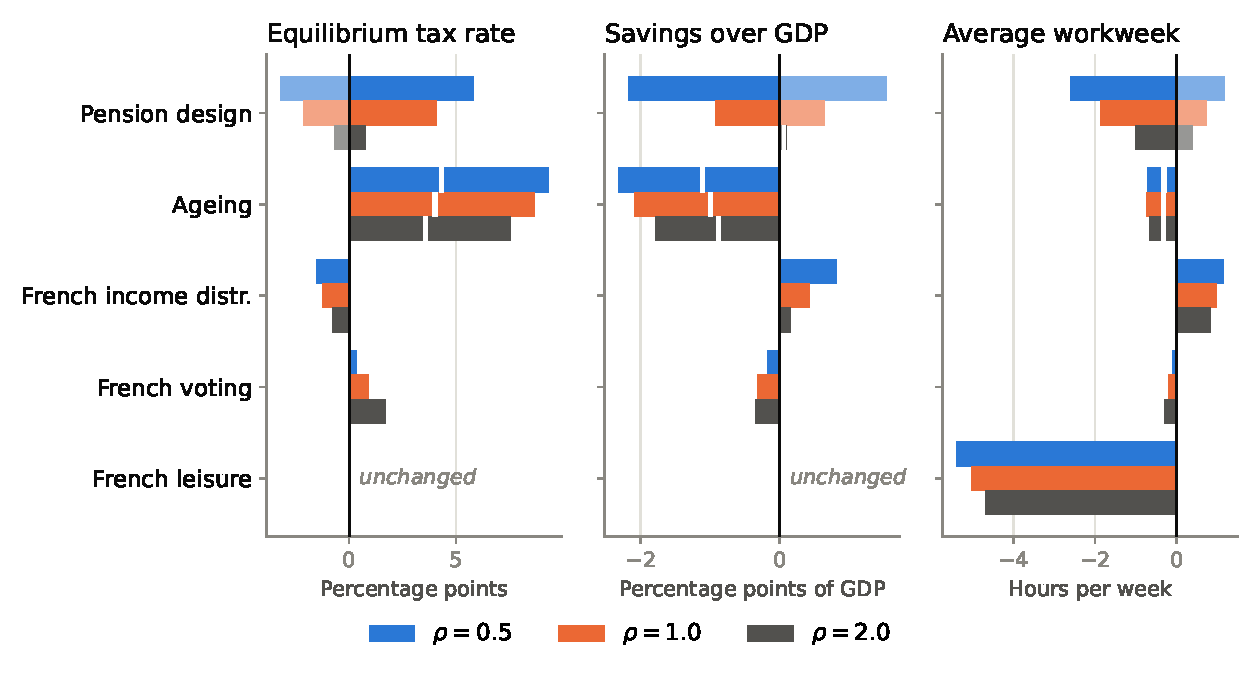
\includegraphics[width=\linewidth]{Figs/US_overview.pdf}\par
\begin{tablenotes}[flushleft]\footnotesize
    \item[] \textit{Note:} Every panel is the deviation from the calibrated U.S.\ baseline at the same $\rho$, whose levels are the baseline rows of table \ref{table:US:CRRA:pensChars}. The savings rate is savings relative to GDP.
\end{tablenotes}
\end{threeparttable}
\end{figure}

\smalltitle{The effect of the intertemporal elasticity of substitution.}
Under general CRRA preferences, with $\rho$ read as the IES as in section \ref{sec:argentina} and each $\rho$ calibrated separately, most counterfactuals change little, and log preferences remain the benchmark (appendix \ref{app:US:CRRA}). Acute ageing raises the tax rate by between $7.6$ and $9.3$ p.p.\ across $\rho \in \{0.5, 1, 2\}$, in line with \textcite{mkvss08}, and France's income distribution moves it several times less at every $\rho$. The exception is pension design: going from $\theta = 1$ to $\theta = 0$ raises the tax rate by $9.0$, $6.2$ and $1.5$ p.p.\ at $\rho = 0.5$, $1$ and $2$ (table \ref{table:US:CRRA:pensChars}). The reason for this is that a higher IES lowers the young's resistance to taxation, so the calibration needs a lower political weight of the old to match the observed tax rate, and the difference in benefits between rich and poor retirees, through which $\theta$ moves the tax rate, counts for less; the savings rate and the workweek follow. Among France's characteristics, only the voting profile has an effect that grows with the IES, from a rise in the tax rate of $0.3$ p.p.\ at $\rho = 0.5$ to $1.7$ p.p.\ at $\rho = 2$ (table \ref{table:US:CRRA:otherShocks}): it raises the weight of the poor young and the poor old alike, and at a higher IES the old's demand for a larger system meets less resistance from the young.

The calibrated parameters absorb institutions that the model does not contain. The political weight of the old, $\omega$, stands for the way legislation is introduced, debated and passed, and for constitutional arrangements such as whether the political system is presidential or parliamentary. The taste for leisure, $X$, stands for preferences and also for institutions that shape labor supply, such as unionization, collective bargaining, labor-market regulation and statutory holidays, so the large differences in $X$ across the three countries include these institutional differences.

We now return to figure \ref{fig:US:OECDdata}, in which pension spending and the Bismarckian index both rise as population growth falls, and neither is related to income inequality. With the design given, the model accounts for the pattern in pension spending: ageing is the main determinant of the equilibrium tax rate, and the income distribution moves it several times less.\footnote{On the disposable-income Gini of figure \ref{fig:US:OECDdata}, the U.S., at 0.42, is the third most unequal of the 29 countries, after Mexico and Turkey, and France, at 0.32, is the median.} The relation between the design and population growth suggests that countries respond to ageing by tying benefits more closely to earnings, which a model that holds $\theta$ fixed cannot address. Section \ref{sec:esc} takes it up by letting the electorate choose $\theta$ as well as $\tau$: costless redistribution puts the choice at a corner (section \ref{sec:esc:corner}), and a deadweight cost of redistribution, calibrated on the U.S.\ design, is tested on the UK and France.
